\lecture{Bivariate Data}{bivariate-data}
\section{Bivariate Data}

\title{Bivariate data}
\subtitle{Determining Relationships From Two Related Data Sets}

%\author{Kelly Black}
%\institute{Clarkson University}
\date{16 April 2012}

\begin{frame}
  \titlepage
\end{frame}

\begin{frame}
  \frametitle{Outline}
  \tableofcontents[pausesection,hideothersubsections,sectionstyle=show/hide]
\end{frame}



\subsection{Clicker Quiz}

\begin{frame}{Clicker Quiz}

  \iftoggle{clicker}{%

    Suppose that \\
    \begin{tabular}{r@{~$=$~}l}
      $x$ & Age of Cat (between 0 and 1 year)  \\
      $y$ & Mass of Cat (kg)
    \end{tabular}

    \vfill

    If $x$ increases what do you expect to happen to $y$?

    \vfill 


    \begin{tabular}{l@{\hspace{3em}}l@{\hspace{3em}}l@{\hspace{3em}}l}
      A: $y$ tends to inc.  & B: No trend & C: $y$ tends to dec.
    \end{tabular}

    \vfill
    \vfill
    \vfill

  }

\end{frame}

\subsection{Bivariate Data}


\begin{frame}
  \frametitle{Bivariate Data}

  \begin{tabular}{r@{~$=$~}l}
    $x$ & Age of Cat (between 0 and 1 year)  \\
    $y$ & Mass of Cat (kg)
  \end{tabular}
  
  \vfill

  \only<2->
  {

    As the age of the cat increases in the first year we expect that
    the cat's mass will \textbf{tend} to increase.

  }

  \only<3->
  {
    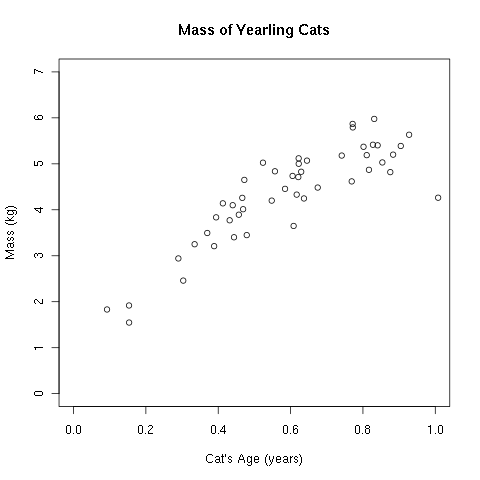
\includegraphics[width=6cm]{img/catsmass}
  }

  \vfill


\end{frame}


\begin{frame}
  \frametitle{Bivariate Data}

  What if we change it a little bit: \\
  \begin{tabular}{r@{~$=$~}l}
    $x$ & Age of Cat (between 0 and 20 years)  \\
    $y$ & Mass of Cat (kg)
  \end{tabular}
  
  \vfill

  \only<2->
  {

    As the age of the cat increases in the first year we expect that
    the cat's mass will \textbf{tend} to increase, but eventually it
    will level out.

  }

  \only<3->
  {
    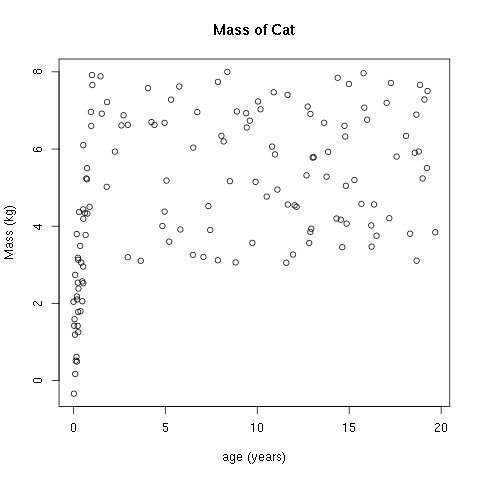
\includegraphics[width=6cm]{img/catsmassLater}
  }

  \vfill


\end{frame}


\begin{frame}
  Question: How do we quantify the ``tendency'' of this relationship?
\end{frame}


\subsection{Correlation}


\begin{frame}
  \frametitle{Define the terms}

  \begin{columns}
    \column{.25\textwidth}

    \begin{tabular}{l|l}
      $X$ & $Y$ \\ \hline
      $x_1$ & $y_1$ \\
      $x_2$ & $y_2$ \\
      $x_3$ & $y_3$ \\
      $x_4$ & $y_4$ \\
      $\vdots$ & $\vdots$ \\
      $x_n$ & $y_n$ \\
    \end{tabular}


    \vfill

    \column{.75\textwidth}

    \only<3->
    {
      There is a ``one to one'' correspondence between each
      row. i.e. $x_3$ and $y_3$ are related to one another.

    }

    \vfill

  \end{columns}


  \begin{columns}
    \column{.5\textwidth}

    \only<4-> {

      Examine $x$ by itself: \\
      \begin{tabular}{l}
        N \\
        $\bar{x}$ \\
        $s_x$
      \end{tabular}

      Standard statistics.

    }
      
    \column{.5\textwidth}


    \only<5-> {

      Examine $y$ by itself: \\
      \begin{tabular}{l}
        N \\
        $\bar{y}$ \\
        $s_y$
      \end{tabular}

      Standard statistics.


    }


  \end{columns}


\end{frame}

\begin{frame}
  \frametitle{Example}

  \begin{columns}
    \column{.25\textwidth}

    \begin{tabular}{l|l}
      $X$ & $Y$ \\ \hline
      1 & 2 \\
      2 & 4  \\
      3 & 9 \\
      4 & 12
    \end{tabular}


    \vfill

    \column{.75\textwidth}

    \only<4->
    {
      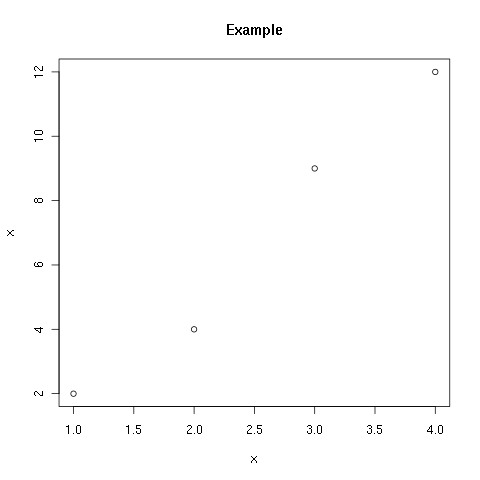
\includegraphics[width=4cm]{img/simpleCorrelationExample}
    }

    \vfill

  \end{columns}


  \begin{columns}
    \column{.5\textwidth}

    \only<2-> {

      Examine $x$ by itself: \\
      \begin{tabular}{l}
        $N=4$ \\
        $\bar{x}=2.5$ \\
        $s_x=1.29$
      \end{tabular}


    }
      
    \column{.5\textwidth}


    \only<3-> {

      Examine $y$ by itself: \\
      \begin{tabular}{l}
        $n=4$ \\
        $\bar{y}=6.75$ \\
        $s_y=4.57$
      \end{tabular}



    }


  \end{columns}


\end{frame}

\begin{frame}{Now Bring Them Together}

  Graphically, we can look at the scatter plot:

  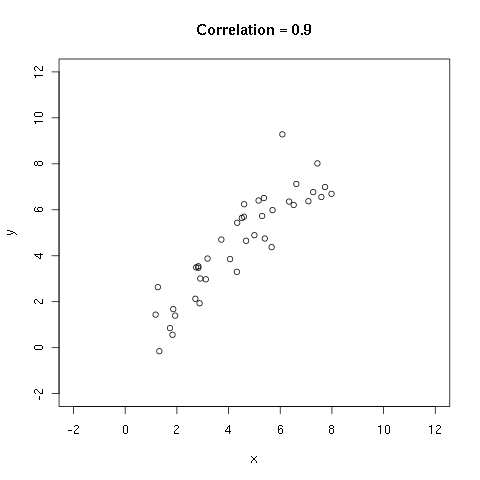
\includegraphics[height=4cm]{img/correlation09}
  
\end{frame}



\begin{frame}{Positive vs. Negative Relationships}

  \begin{columns}
    \column{.45\textwidth}

    \begin{definition}
      If $y$ \textbf{tends} to increase as $x$ increases then we say
      that it is a \textit{positive relationship} : \\
      \centerline{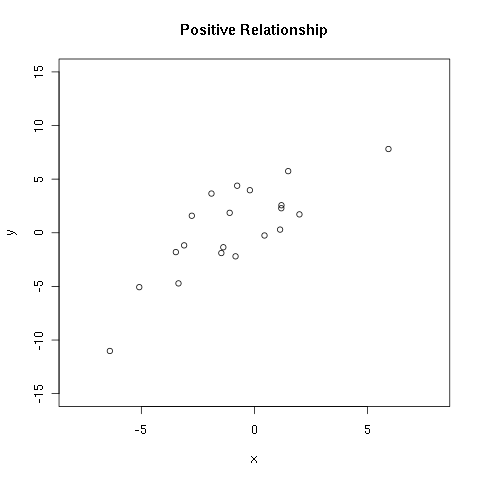
\includegraphics[width=5cm]{img/positiveRelationship}}
    \end{definition}

    \column{.5\textwidth}

    \begin{definition}
      If $y$ \textbf{tends} to decrease as $x$ increases then we say
      that it is a \textit{negative relationship} : \\
      \centerline{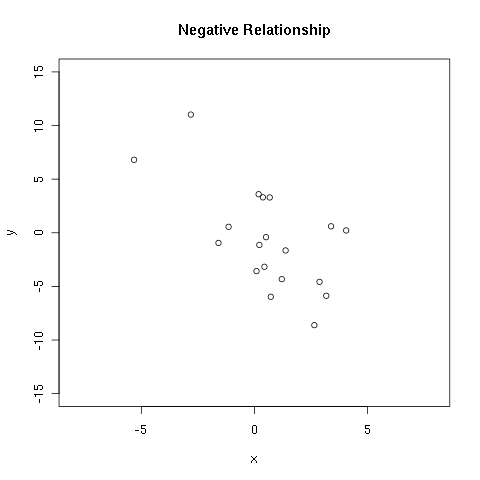
\includegraphics[width=5cm]{img/negativeRelationship}}
    \end{definition}

  \end{columns}
  
\end{frame}


\begin{frame}{Calculating the Correlation}

  First define the following sums:
  \begin{eqnarray*}
    S_{xx} & = & (x_1-\bar{x})^2 + (x_2-\bar{x})^2 + \cdot + (x_n-\bar{x})^2, \\
    S_{yy} & = & (y_1-\bar{y})^2 + (y_2-\bar{y})^2 + \cdot + (y_n-\bar{y})^2, \\
    S_{xy} & = & (x_1-\bar{x}) + (x_2-\bar{x}) + \cdot + (x_n-\bar{x}), \\
  \end{eqnarray*}

  \uncover<2->
  {
    
    \begin{definition}{Sample Correlation}
      The sample correlation coefficient is defined to be
      \begin{eqnarray*}
        r & = & \frac{S_{xy}}{\sqrt{S_{xx} S_{yy}}}.
      \end{eqnarray*}
    \end{definition}

  }
  
\end{frame}


\begin{frame}
  \frametitle{Example}
  \vspace*{-1em}
  \begin{columns}
    \column{.25\textwidth}

    \begin{tabular}{l|l}
      $X$ & $Y$ \\ \hline
      1 & 2 \\
      2 & 4  \\
      3 & 9 \\
      4 & 12
    \end{tabular}


    \vfill

    \column{.75\textwidth}

    \only<2->
    {
      \begin{eqnarray*}
        \bar{x} & = & 2.5 \\
        \bar{y} & = & 6.75
      \end{eqnarray*}
    }

    \vfill

  \end{columns}

  \only<3->
  {
    \begin{eqnarray*}
      s_{xx} & = & \lp 1-2.5\rp^2 + \lp 2 - 2.5 \rp^2 + \lp 3 - 2.5 \rp^2 + \lp 4 - 2.5 \rp^2 \\
            & = & 5, \\
      s_{yy} & = & \lp 2-6.75\rp^2 + \lp 4 - 6.75 \rp^2 + \lp 9 - 6.75 \rp^2 + \lp 12 - 6.75 \rp^2 \\
            & = & 62.75, \\
      s_{xx} & = & \lp 1-2.5\rp\lp 2-6.75\rp + \lp 2 - 2.5 \rp\lp 4 - 6.75 \rp + \lp 3 - 2.5 \rp\lp 9 - 6.75 \rp + \lp 4 - 2.5 \rp\lp 12 - 6.75 \rp \\
            & = & 17.5
    \end{eqnarray*}
  } 

  \only<4->
  {
    \begin{eqnarray*}
      r & = & \frac{17.5}{\sqrt{5\cdot 62.75}}, \\
        & \approx & 0.988
    \end{eqnarray*}
  }


\end{frame}



\begin{frame}{Correlation}

  \hspace*{-3em}
  \begin{tabular}{rrr}
    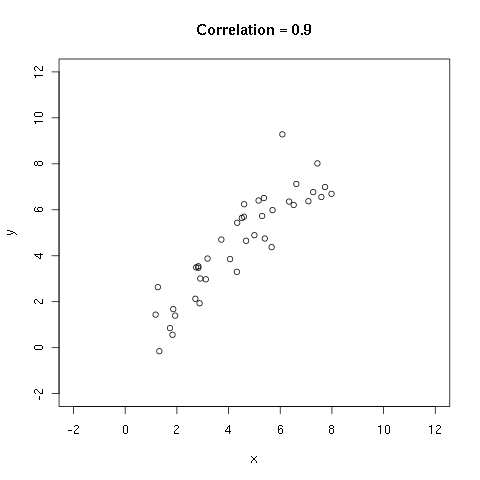
\includegraphics[height=4cm]{img/correlation09} & 
    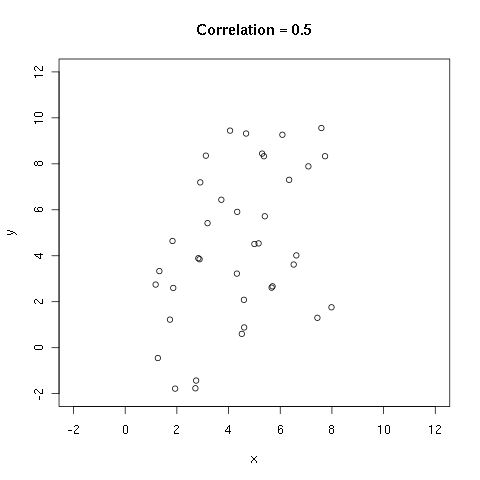
\includegraphics[height=4cm]{img/correlation05} &
    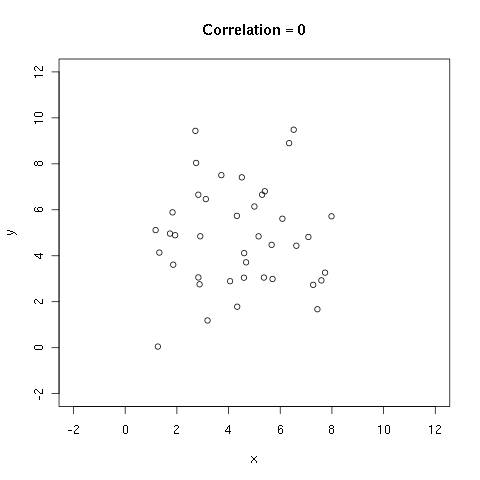
\includegraphics[height=4cm]{img/correlation0} \\
    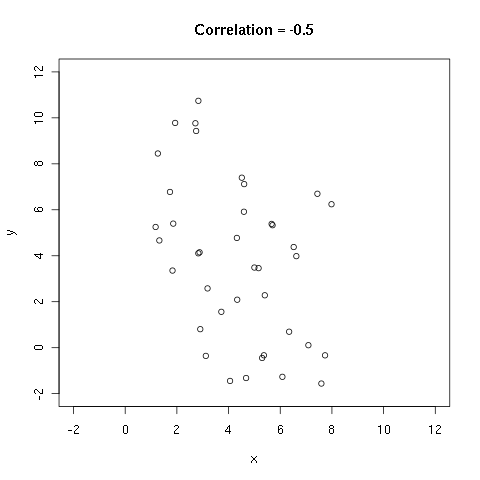
\includegraphics[height=4cm]{img/correlation-05} &
    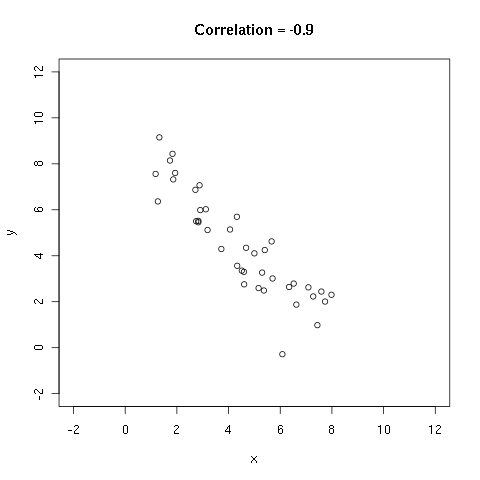
\includegraphics[height=4cm]{img/correlation-09}
  \end{tabular}


\end{frame}


\begin{frame}
  \frametitle{Inference on the Correlation}

  \begin{definition}
    The sample correlation can be used to define a $t$-distribution:
    \begin{eqnarray*}
      t & = & \frac{r\sqrt{n-2}}{\sqrt{1-r^2}}
    \end{eqnarray*}
    with $n-2$ degrees of freedom.
  \end{definition}

\end{frame}

\begin{frame}{Hypothesis Test for the Correlation}

  Is there a relationship between the two variables? \\
  \begin{tabular}{ll}
    $H_0$ & $r=0$, \\
    $H_a$ & $r\neq 0$.
  \end{tabular}

  (Note, a one sided test can also be constructed if you ask if there
  is a positive or negative relationship between the variables.)

  
\end{frame}


\begin{frame}{Clicker Quiz}

  \iftoggle{clicker}{%


    \begin{columns}
      \column{.25\textwidth}

      \begin{tabular}{l|l}
        $X$ & $Y$ \\ \hline
        1 & 2 \\
        2 & 4  \\
        3 & 9 \\
        4 & 12
      \end{tabular}


      \vfill

      \column{.75\textwidth}
      
      \begin{tabular}{ll}
        $H_0$ & $r=0$, \\
        $H_a$ & $r\neq 0$.
      \end{tabular} \\
      Use a 95\% confidence level.

    \vfill

  \end{columns}


    \vfill 


    \begin{tabular}{l@{\hspace{3em}}l@{\hspace{3em}}l@{\hspace{3em}}l}
      A: Reject $H_0$  & B: Do not reject $H_0$
    \end{tabular}

    \vfill
    \vfill
    \vfill

  }

\end{frame}


% LocalWords:  Clarkson pausesection hideallsubsections
